\documentclass[a4paper, 14pt]{extarticle}

%%% Преамбула %%%

\usepackage{fontspec} % XeTeX
\usepackage{xunicode} % Unicode для XeTeX

%\usepackage[T2A,T1]{fontenc}
%\usepackage[utf8]{inputenc}
%\usepackage[russian,english]{babel}

\defaultfontfeatures{Ligatures=TeX}
\setmainfont{Times New Roman} % Нормоконтроллеры хотят именно его
\newfontfamily\cyrillicfont{Times New Roman}

\usepackage{polyglossia}
\setdefaultlanguage{russian}

% Отступы у страниц
\usepackage{geometry}
\geometry{
	left=3cm,
	right=1.5cm,
	top=2cm,
	bottom=2cm
}

\renewcommand{\baselinestretch}{1.5} % Полуторный межстрочный интервал
\setlength{\parindent}{5ex} % Абзацный отступ
\setlength{\parskip}{0.3cm} % Расстояние между абзацами

\usepackage{indentfirst} % Красная строка после заголовка

% Многоточие в оглавлении
\usepackage{tocloft}
\renewcommand{\cftsecleader}{\cftdotfill{\cftdotsep}}


%\usepackage[center]{titlesec} % Центрирование заголовков
%\titleformat{\section}
%  {\centering\large\bfseries} % format
%  {}% label
%  {0pt} % sep
%  {\large}

%\titleformat{\subsection}
%  {\normalsize\bfseries} % format
%  {}% label
%  {0pt} % sep
%  {\normalsize}

% Центрирование заголовков
%\usepackage{sectsty}
%\sectionfont{\centering}

% Списки
\usepackage{enumitem}
\setlist[enumerate,itemize]{leftmargin=12.7mm} % Отступы в списках

\makeatletter
    \AddEnumerateCounter{\asbuk}{\@asbuk}{м)}
\makeatother
\setlist{nolistsep} % Нет отступов между пунктами списка

\usepackage{unicode-math}
\usepackage{amsmath}
%\usepackage{amssymb}
\numberwithin{equation}{section}

\renewcommand{\contentsname}{\centering{Содержание}}

\begin{document}

\begin{titlepage}
  \thispagestyle{empty}
  \begin{center}
  {
    \fontsize{16}{16}
    \selectfont
    \noindent
    МИНИСТЕРСТВО ОБРАЗОВАНИЯ И НАУКИ \\
    РОССИЙСКОЙ ФЕДЕРАЦИИ \\
    ФЕДЕРАЛЬНОЕ ГОСУДАРСТВЕННОЕ БЮДЖЕТНОЕ \\
    ОБРАЗОВАТЕЛЬНОЕ УЧЕРЕЖДЕНИЕ \\
    ВЫСШЕГО ОБРАЗОВАНИЯ \\
    <<ВОРОНЕЖСКИЙ ГОСУДАРСТВЕННЫЙ УНИВЕРСИТЕТ>> \\
    (ФГБОУ ВО <<ВГУ>>) \\
    ФАКУЛЬТЕТ ПРИКЛАДНОЙ МАТЕМАТИКИ, \\
    ИНФОРМАТИКИ И МЕХАННИКИ
  }

  \vspace{2cm}

  {
    \fontsize{16}{16}
    \selectfont
    \textbf{ОТЧЁТ}

    По работе <<Решение статической задачи теплопроводности \\
    методом конечных элементов>>
  }

  \vfill

  \begin{flushright}
    Выполнили: студенты 1 курса магиструтры \\
    11 группы \\
    Васильев Н.А. \\
    Малик М.С. \\
    Польшаков Д.В. \\
    Токарев М.И. \\
    Проверила: \\
    доц. Корзунина В.В.
  \end{flushright}

  \vfill

  г. Воронеж, \the\year
  \end{center}
\end{titlepage}

\clearpage


\setcounter{page}{2} % Начало нумерации страниц

\tableofcontents

\clearpage

\section{Постановка задачи}

Методом конечных элементов численно реализовать решение уравнения
теплопроводности \ref{eq:heat} с граничными условиями первого и третьего рода.

\begin{equation}
\partial/\partial x \left(k_x(x,y) \frac{du}{dx} \right) +
\partial/\partial x \left(k_y(x,y) \frac{du}{dy}\right) = f(x,y)
\end{equation} \label{eq:heat}

Уравнение решается в прямоугольной области, которая разбивается на
прямоугольники с диагоналями "юго-запад - северо-восток". Треугольные элементы
линейные, при численном интегрировании используется схема второго порядка
точности. Полученное распределение температуры выводится в файл и представляется
графически (тональное раскрашивание).

\clearpage

\section{Входные данные}

\begin{itemize}
	\item $N_x, N_y$ --  количество точек разбиения по направлению x,y;
	\item $h_x[0 .. N_x-1], h_y[0 .. N_y-1]$ -- массивы шагов по x,y;
	\item $X_0, Y_0$ -- координата левого нижнего угла прямоугольной области;
	\item $k_x(x,y), k_y(x,y), f(x,y)$ -- коэффициенты уравнения;
	\item $\varphi(x,y)$ -- функция, задающая граничное условие.
\end{itemize}

\clearpage
\section{Теоретический материал}

\subsection{Метод конечных элементов}

Суть метода заключена в его названии. Область, в которой ищется решение
дифференциальных уравнений, разбивается на конечное количество подобластей
(элементов). В каждом из элементов произвольно выбирается вид аппроксимирующей
функции. В простейшем случае это полином первой степени. Вне своего элемента
аппроксимирующая функция равна нулю. Значения функций на границах элементов (в
узлах) являются решением задачи и заранее неизвестны. Коэффициенты
аппроксимирующих функций обычно ищутся из условия равенства значения соседних
функций на границах между элементами (в узлах). Затем эти коэффициенты
выражаются через значения функций в узлах элементов. Составляется система
линейных алгебраических уравнений. Количество уравнений равно количеству
неизвестных значений в узлах, на которых ищется решение исходной системы, прямо
пропорционально количеству элементов и ограничивается только возможностями ЭВМ.
Так как каждый из элементов связан с ограниченным количеством соседних, система
линейных алгебраических уравнений имеет разрежённый вид, что существенно
упрощает её решение.

Если говорить в матричных терминах, то собираются так называемые матрицы
жёсткости (или матрица Дирихле) и масс. Далее на эти матрицы накладываются
граничные условия (например, при условиях Неймана в матрицах не меняется ничего,
а при условиях Дирихле из матриц вычёркиваются строки и столбцы, соответствующие
граничным узлам, так как в силу краевых условий значение соответствующих
компонент решения известно). Затем собирается система линейных уравнений и
решается одним из известных методов.

С точки зрения вычислительной математики, идея метода конечных элементов
заключается в том, что минимизация функционала вариационной задачи
осуществляется на совокупности функций, каждая из которых определена на своей
подобласти, для численного анализа системы позволяет рассматривать его как одну
из конкретных ветвей диакоптики — общего метода исследования систем путём их
расчленения.

\subsection{Стационарная задача теплопроводности}

Уравнение теплопроводности в сплошной среде имеет вид

\begin{equation}
	K_{xx} \frac{\partial^2 T}{\partial x^2} +
	K_{yy} \frac{\partial^2 T}{\partial y^2} +
	Q = 0
\end{equation} \label{eq:heat}

где $T$ – температура; $K_{xx}$, $K_{yy}$ – коэффициенты теплопроводности в
направлениях $x$, $y$, $z$ размерности $ \text{кВт/м} \cdot \text{K} $; $Q$ –
источник тепла внутри тела, который считается положительным, если тепло
подводится к телу, его размерность $\text{кВт/м}^2$. С уравнением \ref{eq:heat}
связано граничное условие первого рода. Если температура известна на некоторой
части границы, то пишут

\begin{equation}
	T = T_B(s)
\end{equation}

где $T_B$ – температура на границе, которая может быть функцией координат точек
поверхности $s$. Матрица теплопроводности элемента имеет вид:

\begin{equation}
	[k^{(e)}] =
	\int\limits_{S^{(e)}} [B^{(e)}]^T [D^{(e)}] dV
\end{equation}

Матрица $[N^{(e)}]$ содержит функции формы, причем

\begin{equation}
	T^{(e)} = [N^{(e)}]\{T\}
\end{equation}

Матрица $[D^{(e)}]$ содержит значения коэффициентов теплопроводности:

\begin{equation}
	[D^{(e)}] = \begin{bmatrix}
		K_{(e)}^{xx} & 0            \\
		0            & K_{(e)}^{xx} \\
	\end{bmatrix}
\end{equation}

а матрица $[B^{(e)}]$ получается дифференцированием $[N^{(e)}]$ по $x$, $y$ и
$z$. Соотношение для определения $[B^{(e)}]$ имеет вид

\begin{equation}
	\{g\} = \begin{Bmatrix}
	\frac{\partial T}{\partial x} \\
	\frac{\partial T}{\partial y}
	\end{Bmatrix} = [B^{(e)}]\{T\}
\end{equation}


Вектор-столбец правых частей уравнений для элемента определяется формулой:
\begin{equation}
	\{f^{(e)}\} = - \int\limits_{S^{(e)}} [N^{(e)}]^T QdV
\end{equation}

\clearpage
\section{Средства реализации}

Реализация поставленной задачи была выполнина с использованием языка
программирования C++. В качестве среды разработки выбрана Qt Creator.

Для отрисовки результата вычислений используется технология OpenGL. Для
отображения его на форме выбрана библиотека Qt.

Для проверки работоспособности программных модулей были разработаны
автоматизированные тесты с использованием библиотеки cppunit

\clearpage
\section{Пример работы программы}

\begin{figure}[h]
	\centering
	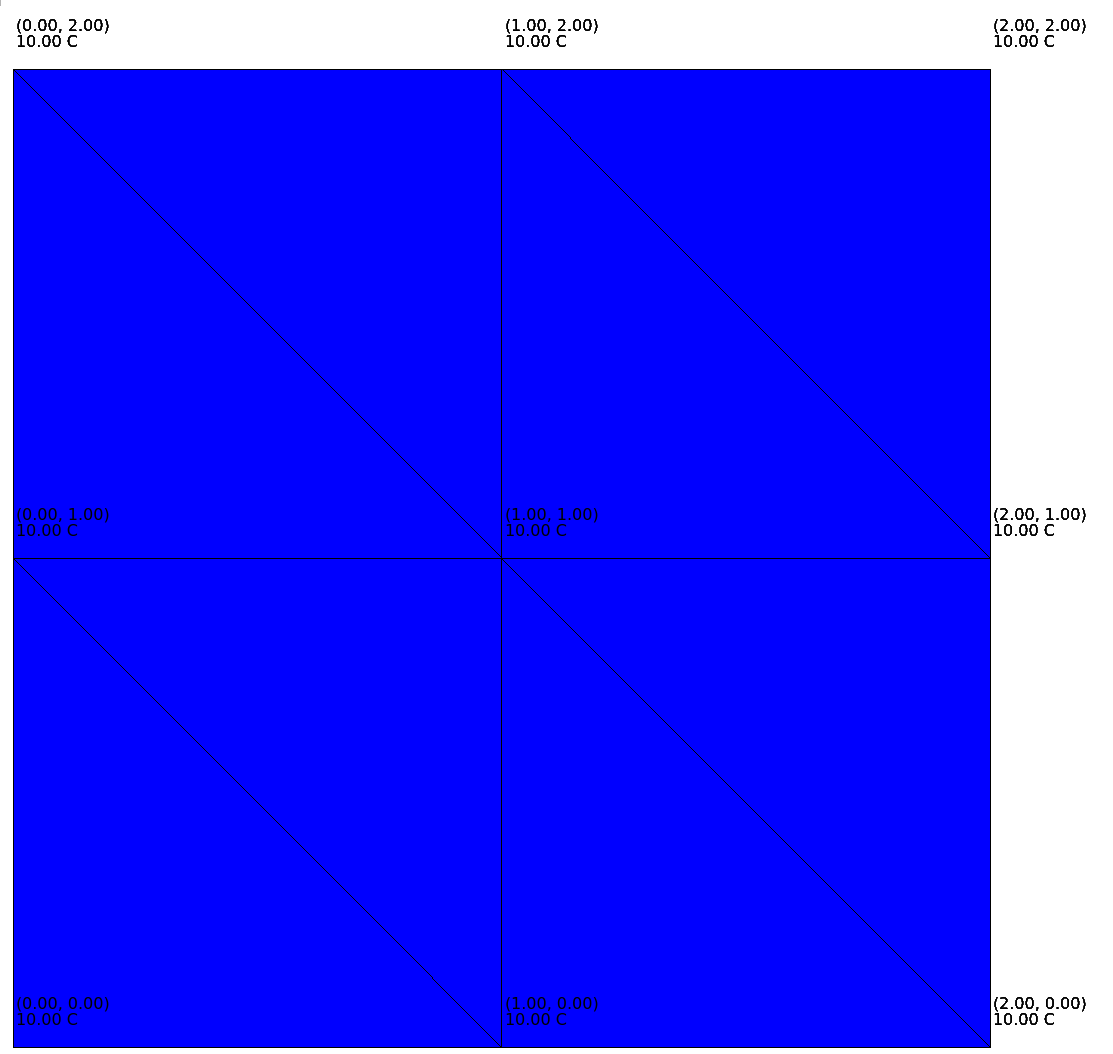
\includegraphics[width=0.7\linewidth]{images/test1}
	\caption[Рисунок]{Постоянная функция}
\end{figure}

\begin{figure}[h]
	\centering
	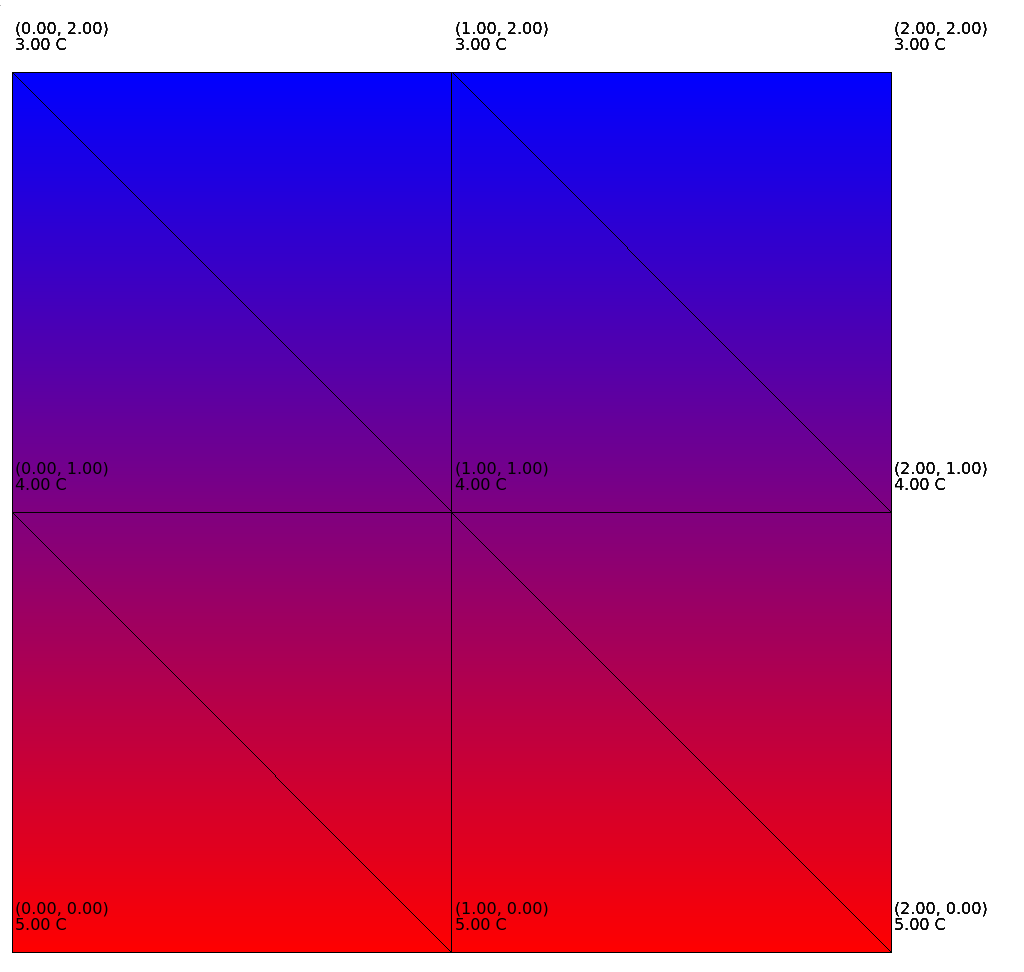
\includegraphics[width=0.7\linewidth]{images/test2}
	\caption[Рисунок]{Линейная функция}
\end{figure}

\begin{figure}[h]
	\centering
	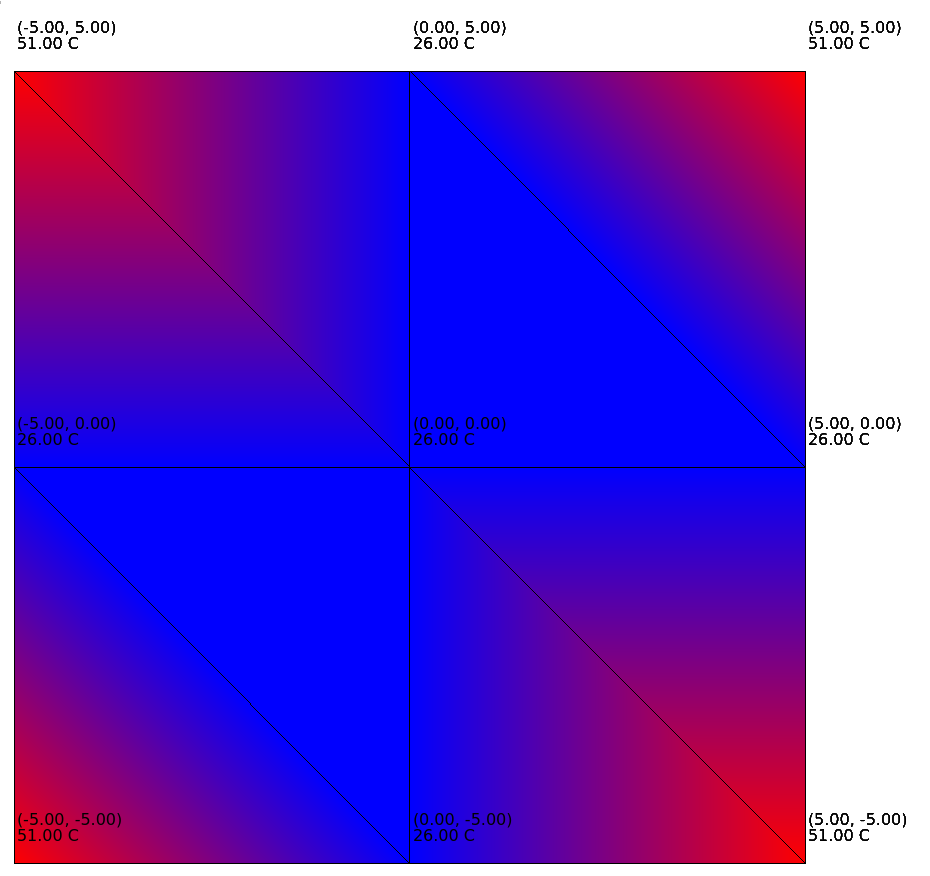
\includegraphics[width=0.7\linewidth]{images/test3}
	\caption[Рисунок]{Квадратичная функция}
\end{figure}

\begin{figure}[h]
	\centering
	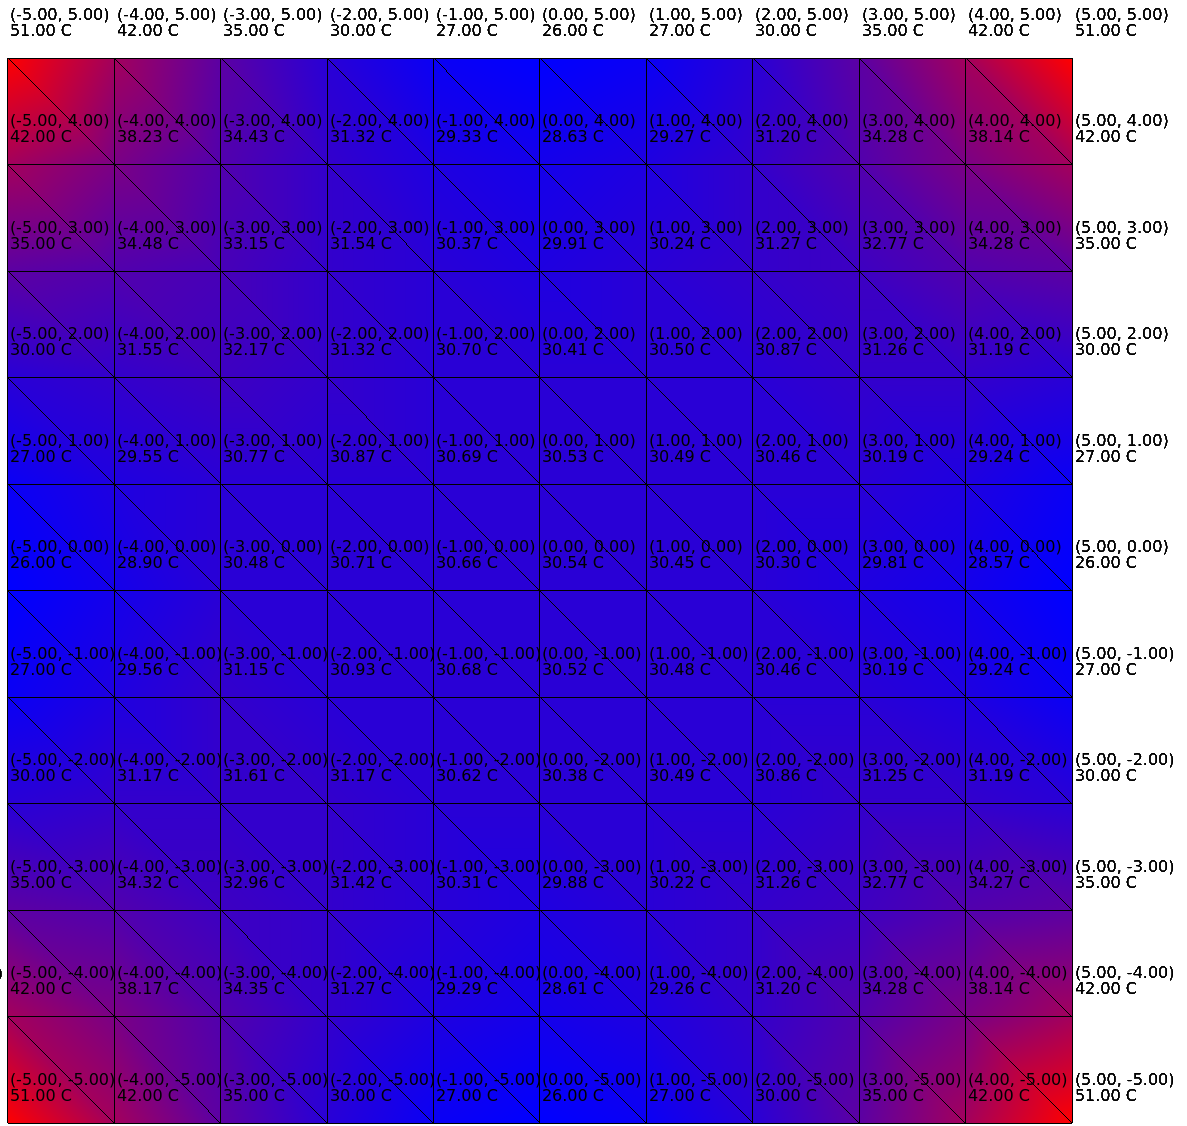
\includegraphics[width=0.7\linewidth]{images/test4}
	\caption[Рисунок]{Квадратичная функция с более частым разбиением}
\end{figure}


\clearpage
\section{Заключение}

В результате данной работы было реализовано приложение, которое решает плоскую
стационарную задачу теплопроводности в прямоугольной области для тел с
переменными коэффициентами теплопроводности. А также реализовано графическое
приложение, которое позволяет осуществлять выбор входных данных  и визуализирует
решение задачи на заданной прямоугольной области.

\end{document}
